\documentclass[aspectratio=169]{beamer}

% Required packages
\usepackage{tikz}
\usepackage{listings}
\usepackage{xcolor}

% Define Star Trek DS9 color scheme
\definecolor{ds9blue}{RGB}{25,25,112}
\definecolor{ds9gold}{RGB}{218,165,32}
\definecolor{ds9grey}{RGB}{105,105,105}
\definecolor{ds9red}{RGB}{178,34,34}

% Theme configuration
\usetheme{Madrid}
\usecolortheme[named=ds9blue]{structure}
\setbeamercolor{alerted text}{fg=ds9red}
\setbeamercolor{example text}{fg=ds9gold}

% Code listing style
\lstset{
    language=C++,
    basicstyle=\small\ttfamily,
    keywordstyle=\color{ds9blue},
    commentstyle=\color{ds9grey},
    stringstyle=\color{ds9gold},
    numbers=left,
    numberstyle=\tiny\color{ds9grey},
    frame=single,
    breaklines=true
}

% Title page configuration
\title[Arrays in C++]{PHYS11 CH: Array Fundamentals}
\subtitle{Memory, Functions, and Safety in C++}
\author[Mr. Gullo]{Mr. Gullo}
\date[Fall 2024]{Fall Semester 2024}
\institute[Physics Dept.]{Department of Physics \\ Advanced Programming Division}

\begin{document}

\begin{frame}
    \titlepage
\end{frame}

\begin{frame}
    \frametitle{Learning Objectives}
    By the end of this presentation, you will understand:
    \begin{itemize}[<+->]
        \item \textbf{Array Fundamentals}
        \begin{itemize}
            \item Declaration, initialization, and access patterns
            \item Memory layout and sequential storage
        \end{itemize}
        \item \textbf{Array Functions}
        \begin{itemize}
            \item Passing arrays as parameters
            \item Creating utility functions for array operations
        \end{itemize}
        \item \textbf{Memory Safety}
        \begin{itemize}
            \item Pointer arithmetic and memory layout
            \item Best practices for array bounds
        \end{itemize}
    \end{itemize}
\end{frame}

\section{Array Fundamentals}

\begin{frame}[fragile]
    \frametitle{Array Declaration \& Initialization}
    \begin{columns}
        \column{0.6\textwidth}
        From Code Base 1:
        \begin{lstlisting}
int aOne[] = {1, 2, 3, 4, 5, 
              6, 7, 8, 9, 10};
int length = 10;
        \end{lstlisting}
        \column{0.4\textwidth}
       
    \end{columns}
    \pause
    \begin{itemize}
        \item Arrays are \alert{contiguous} blocks of memory
        \item Index starts at \textbf{0}
        \item Size can be implicit or explicit
    \end{itemize}
\end{frame}

\begin{frame}[fragile]
    \frametitle{Array Access \& Traversal}
    From Code Base 1:
    \begin{lstlisting}
// accessing elements
cout << aOne[0];  // first element
cout << aOne[length-1];  // last element

// traversal pattern
for(int i=0; i < length; i++)
    cout << aOne[i] << ", ";
    \end{lstlisting}
    \pause
    \begin{alertblock}{Key Points}
        \begin{itemize}
            \item Array indices range from \textbf{0} to \textbf{length-1}
            \item Common pattern: loop with counter variable
            \item Direct access with square bracket notation
        \end{itemize}
    \end{alertblock}
\end{frame}

\section{Array Functions}

\begin{frame}[fragile]
    \frametitle{Functions with Arrays}
    From Code Base 2:
    \begin{lstlisting}
void printArray(int arr[], int first, int last){
   if(first <= last)
      cout << arr[first];
   for(int i = first + 1; i <= last; i++)
      cout << ", " << arr[i];
}
    \end{lstlisting}
    \pause
    \begin{exampleblock}{Function Parameters}
        \begin{itemize}
            \item Arrays decay to pointers when passed
            \item Size must be passed separately
            \item Original array can be modified
        \end{itemize}
    \end{exampleblock}
\end{frame}

\begin{frame}[fragile]
    \frametitle{Array Size Determination}
    From Code Base 2:
    \begin{lstlisting}
// Getting array size
int aOneLength = sizeof(aOne)/sizeof(aOne[0]);

// Fixed size declaration
const int aTwoLength = 10;
int aTwo[aTwoLength];
    \end{lstlisting}
    \pause
    \begin{columns}
        \column{0.6\textwidth}
        \begin{itemize}
            \item sizeof operator gives total bytes
            \item Division gives element count
            \item const for fixed-size arrays
        \end{itemize}
        \column{0.4\textwidth}
        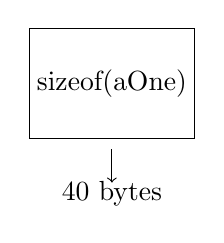
\begin{tikzpicture}[scale=0.7]
            \draw (0,0) rectangle (3,-2);
            \node at (1.5,-1) {sizeof(aOne)};
            \draw[->] (1.5,-2.2) -- (1.5,-2.8);
            \node at (1.5,-3) {40 bytes};
        \end{tikzpicture}
    \end{columns}
\end{frame}

\section{Memory Safety}

\begin{frame}[fragile]
    \frametitle{Pointer Arithmetic}
    From Code Base 3:
    \begin{lstlisting}
int *aAdd = &aArr[1];  // Address of second element
int *bAdd = &bArr[1];  // Address of second element

if(aAdd < bAdd) {
    // Calculate distance between arrays
    for(int i = 0; i < bAdd - aAdd + length; i++)
        cout << aArr[i] << ", ";
}
    \end{lstlisting}
    \pause
    \begin{alertblock}{Warning}
        Accessing memory beyond array bounds leads to undefined behavior!
    \end{alertblock}
\end{frame}

\begin{frame}
    \frametitle{Memory Layout Visualization}
    \begin{center}
        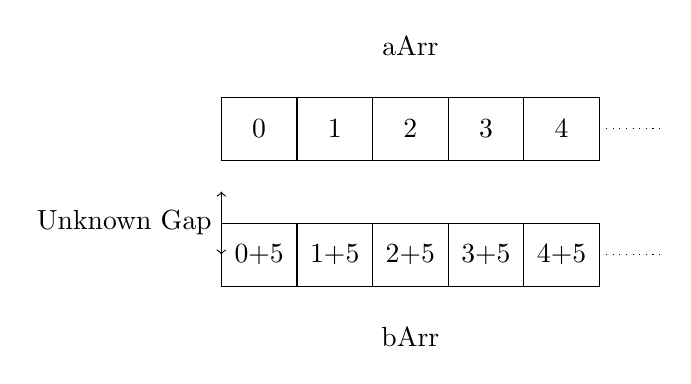
\begin{tikzpicture}[scale=0.8]
            % First array
            \foreach \x in {0,...,4} {
                \draw (\x*1.2,0) rectangle ++(1.2,1);
                \node at (\x*1.2+0.6,0.5) {\x};
            }
            \node[above] at (3,1.5) {aArr};
            
            % Second array
            \foreach \x in {0,...,4} {
                \draw (\x*1.2,-2) rectangle ++(1.2,1);
                \node at (\x*1.2+0.6,-1.5) {\x+5};
            }
            \node[below] at (3,-2.5) {bArr};
            
            % Memory gap illustration
            \draw[dotted] (6,0.5) -- (7,0.5);
            \draw[dotted] (6,-1.5) -- (7,-1.5);
            
            \draw[<->] (0,-0.5) -- (0,-1.5) 
                node[midway,left] {Unknown Gap};
        \end{tikzpicture}
    \end{center}
    \pause
    \begin{itemize}
        \item Arrays may not be adjacent in memory
        \item Gap size is implementation-dependent
        \item Never assume array positions
    \end{itemize}
\end{frame}

\section{Modern C++ Considerations}

\begin{frame}
    \frametitle{Best Practices}
    \begin{columns}
        \column{0.5\textwidth}
        \textbf{Traditional Arrays}
        \begin{itemize}
            \item No bounds checking
            \item Size must be tracked
            \item Pointer decay issues
            \item Manual memory management
        \end{itemize}
        
        \column{0.5\textwidth}
        \textbf{Modern Alternatives}
        \begin{itemize}
            \item std::array
            \item std::vector
            \item Automatic bounds checking
            \item Size tracking built-in
        \end{itemize}
    \end{columns}
    \pause
    \begin{alertblock}{Safety First}
        Always prefer standard container classes for production code!
    \end{alertblock}
\end{frame}

\begin{frame}
    \frametitle{Summary}
    \begin{itemize}[<+->]
        \item Arrays provide sequential memory storage
        \item Access and traversal patterns are fundamental
        \item Functions receive arrays as pointers
        \item Memory safety requires careful consideration
        \item Modern C++ offers safer alternatives
    \end{itemize}
    \pause
    \begin{exampleblock}{Key Takeaway}
        Understanding array fundamentals is crucial, but always prioritize safety and modern practices in real applications.
    \end{exampleblock}
\end{frame}

\end{document}